\scanpage{416}

La composition avec la projection can. dans
$T_\rho\times N'_\sigma$ donne un \uline{mono}

\margin{car on aura
\diagram{\begin{tikzcd}[ampersand replacement=\&]
T_0 \arrow[r,"{\substack{\det\\\sim}}"] \& \mathbb G_m
\end{tikzcd}}}

\[
(24)\qquad
\diagram{\begin{tikzcd}[ampersand replacement=\&,column sep=large]
\mathcal T_{\rho,\sigma} \arrow[r,hook] \arrow[d,phantom,"{\rotatebox{90}{$\simeq$}}" description]
 \& T_\rho\times N'_\sigma \\
\left\{(\underline a,\underline b)\mid
 (\det\underline a/\det\underline b)^2=1\right\}
 \& \inserted{\left.\begin{gathered}
\text{i.e. }\det\underline a=\varepsilon'\det\underline b\\
\text{avec }\varepsilon'^2=1
\end{gathered}\right\}}
\end{tikzcd}}
\]

et on aura donc
\[
(25)\qquad
\left\{\begin{aligned}
\chi(\underline a,\underline b)&=\det\underline b\\
\varepsilon_2(\underline a,\underline b)&=\varepsilon_\sigma(\underline b)\\
\varepsilon_3(\underline a,\underline b)&=\det(\underline a)/\det(\underline b)
 =\det\underline b/\det\underline a
\end{aligned}\right.
\]

On définit
\[
(26)\qquad
\diagram{\begin{tikzcd}[ampersand replacement=\&,column sep=small]
\mathcal T_{\rho,\sigma}^{\circ} \arrow[d,phantom,"{\rotatebox{90}{$\simeq$}}" description]
 \& {}=\operatorname{Ker}\mathcal T_{\rho,\sigma}
 \arrow[r,"{(\varepsilon_2,\varepsilon_3)}"]
 \& \mu_2\times\mu_2 \\
\inserted{T_\rho\times_{\mathbb G_m}T_\sigma} \&\&
\end{tikzcd}}
\]
donc on a
\[
(27)\qquad
\diagram{\begin{tikzcd}[ampersand replacement=\&]
1 \arrow[r] \& \mathcal T_{\rho,\sigma}^{\circ} \arrow[r]
 \& \mathcal T_{\rho,\sigma} \arrow[r] \& \mu_2\times\mu_2 \arrow[r] \& 1
\end{tikzcd}}
\]
et une suite exacte canonique
\[
(28)\qquad
\diagram{\begin{tikzcd}[ampersand replacement=\&]
1 \arrow[r] \&
\overbrace{ST_\rho\times ST_\sigma}^{\inserted{\mathcal T_{\rho,\sigma}^{\circ+}}}
\arrow[r] \& \mathcal T_{\rho,\sigma}^{\circ} \arrow[r,"{\chi}"]
 \& \mathbb G_m \arrow[r] \& 1,
\end{tikzcd}}
\]
où on définit
\[
(29)\qquad
\left\{\begin{aligned}
ST_\rho&=\{g\in\Gamma T_\rho\mid\det g=1\}\\
ST_\sigma&=\{g\in\Gamma T_\sigma\mid\det g=1\}
\end{aligned}\right.\quad.
\]

\margin{\figure{\begin{tikzpicture}[x=.65cm,y=.65cm]
\draw[->] (0,4.5) .. controls (1.1,4.55) and (1.1,3.7) .. (1.1,3.25)
 -- (1.2,.8) .. controls (1.2,.45) and (1.55,.55) .. (2.4,.65);
\draw (0,0) .. controls (1.0,-.05) and (1.05,.1) .. (1.15,.45)
 .. controls (1.25,.75) and (1.55,.65) .. (2.4,.65);
\end{tikzpicture}}}
\inserted{L'opération de $\mathcal T_{\rho,\sigma}\simeq
\mathcal M_{\rho,\sigma}(0)$ sur $L_0$ est donnée par
\[
(30)\qquad g(\varepsilon_0(\lambda))=\varepsilon_0(\mu\lambda),
\quad\text{où }\mu=\chi(g)
\]}

On fait opérer $\mathcal M_{\rho,\sigma}(0)
(\simeq\mathcal T_{\rho,\sigma})$ sur $SG$, par
\[
(31)\qquad
\diagram{\begin{tikzcd}[ampersand replacement=\&,column sep=large]
\mathcal M_{\rho,\sigma}(0)
 \arrow[r,"{\text{projection}}"]
 \& T_0 \arrow[r,"{\substack{\text{can.}\\(\text{mono})}}"]
 \& PG \arrow[r,"{\sim}"]
 \& \underline{\operatorname{Aut}}_{\mathrm{gr}}(SG) \\
T_0\times T_\rho\times N'_\sigma \arrow[u,phantom,"{\cap}" description]
 \& G \arrow[u,phantom,"{\cap}" description]
 \& G/\mathbb G_m\simeq\underline{\operatorname{Aut}}(G)
 \arrow[u,phantom,"{\rotatebox{90}{$\simeq$}}" description] \&
\end{tikzcd}}
\]

\par\noindent 415

\scanpage{417}
\mspage{510}

et on définit
\[
(32)\qquad \mathcal M_{\rho,\sigma}\simeq
 \mathcal M_{\rho,\sigma}(0)\mathbin{.}SG
\]
\hfill produit $\frac12$ direct

On a donc un hom can
\[
(33)\qquad
\diagram{\begin{tikzcd}[ampersand replacement=\&]
SG \arrow[r,hook,"{j}"] \& \mathcal M_{\rho,\sigma}
\end{tikzcd}}
\]
dont l'image est notée $\widetilde{\mathcal G}_{\rho,\sigma}^{+}$, donc
\[
(34)\qquad
\diagram{\begin{tikzcd}[ampersand replacement=\&]
1 \arrow[r] \& \widetilde{\mathcal G}_{\rho,\sigma}^{+} \arrow[r]
 \& \mathcal M_{\rho,\sigma} \arrow[r] \& \mathcal T_{\rho,\sigma} \arrow[r] \& 1
\end{tikzcd}}
\]
\[
(35)\qquad
\diagram{\begin{tikzcd}[ampersand replacement=\&,column sep=0.3em,row sep=1.3em]
\mathcal M_{\rho,\sigma}\simeq \& \mathcal M_{\rho,\sigma}(0)
 \arrow[d,phantom,"{\rotatebox{90}{$\simeq$}}" description]
 \& {}\mathbin{.}\widetilde{\mathcal G}_{\rho,\sigma}^{+} \\
 \& \mathcal T_{\rho,\sigma} \&
\end{tikzcd}}
\]
\hfill produit $\frac12$ direct.

\uline{NB.} On utilise la notation $\mathcal T_{\rho,\sigma}$ pour le
groupe quotient
\[
(36)\qquad \mathcal T_{\rho,\sigma}\simeq
\mathcal M_{\rho,\sigma}/\widetilde{\mathcal G}_{\rho,\sigma}^{+},
\]
la notation $\mathcal M_{\rho,\sigma}[0)$ pour le sous-groupe
de $\mathcal M_{\rho,\sigma}$.

On définit un plongement canonique
\[
(37)\qquad
\diagram{\begin{tikzcd}[ampersand replacement=\&]
\mathcal M_{\rho,\sigma}[0] \arrow[r,hook,"{i}"] \& \mathcal M_{\rho,\sigma}
\end{tikzcd}}
\]
qui prolonge les inclusions \unsure{des sous-groupes|du sous-groupe}
$\mathcal M_{\rho,\sigma}(0)$ commun de $\mathcal M_{\rho,\sigma}[0]$
et de $\mathcal M_{\rho,\sigma}$,
et qui sur $L_0$ est donné par
\[
(38)\qquad i(\lambda)=j(\lambda)\qquad (\text{cf }(33))
\]
(ce qui est bien compatible avec les opérations de
$\deleted{\unsure{\mathcal T|\mathcal M}}\mathcal M_{\rho,\sigma}(0)$
sur $L_0$ d'une part, sur $SG\simeq\widetilde{\mathcal G}_{\rho,\sigma}^{+}$
de l'autre).

\par\noindent 416

\scanpage{418}

Une autre façon de le dire, c'est de constater que
$\mathcal M_{\rho,\sigma}(0)$ opérant sur
$SG\simeq\widetilde{\mathcal G}_{\rho,\sigma}^{+}$
normalise le sous-groupe $j(L_0)$ -- que nous
identifions désormais à $L_0$), de sorte qu'on
aura un sous-groupe
\[
\mathcal M_{\rho,\sigma}(0)\mathbin{.}L_0\subset\mathcal M_{\rho,\sigma}
\]
qui \unsure{est|sera} canoniquement isom. à $\mathcal M_{\rho,\sigma}[0]$
défini plus haut, grâce à l'écriture $(\unsure{19|49})$ de
celui-ci comme produit $\frac12$-direct.

\deleted{\uline{Proposition}}
\inserted{\uline{Remarque.}} On a
\[
\deleted{(\unsure{39})}\qquad
\mathcal M_{\rho,\sigma}[0]\subset
\underline{\operatorname{Norm}}_{\mathcal M_{\rho,\sigma}}(L_0)
\]

Par construction, \deleted{\unsure{on a} $\subset$, \unsure{pour} $\unsure{\supset}$}
l'inclusion en sens inverse reviendrait à dire que $L_0$
est son propre normalisateur dans $SG\simeq\widetilde{\mathcal G}_{\rho,\sigma}^{+}$,
ce qui bien sûr n'est pas vrai du tout
-- \unsure{bien} que le fait analogue soit vrai
dans le groupe profini
$\widetilde{\mathcal G}_{0,3}^{\widehat{+}}$,
pour le ss-groupe engendré par $\varepsilon_0$,
ou dans $\Pi_{0,\widehat{3}}$ pour
celui engendré par $l_0$ (\unsure{moyennant} vérification !
d'ailleurs que je n'ai tjrs pas fait).

\par\noindent 417

\scanpage{419}
\mspage{511}

\margin{$\mathcal M_{\rho,\sigma}^{\circ},\mathcal M_{\rho,\sigma}^{+},
\mathcal M_{\rho,\sigma}^{+\circ},\mathcal T_{\rho,\sigma}^{\circ},
\mathcal T_{\rho,\sigma}^{+},\mathcal T_{\rho,\sigma}^{\circ+}\ldots$
quelques sous-groupes centraux et calculs de \unsure{pts} entiers\ldots}

\Needspace{14\baselineskip}
\figure{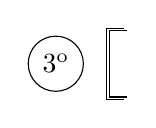
\begin{tikzpicture}[baseline=(n.base)]
\node[draw,circle,inner sep=3pt] (n) at (0,0) {$3^{\mathrm o}$};
\draw[line width=.6pt] (.90,.42)--(.68,.42)--(.68,-.42)--(.90,-.42);
\draw[line width=.45pt] (.86,.45)--(.64,.45)--(.64,-.45)--(.86,-.45);
\end{tikzpicture}}\par\nobreak
On désigne par $\mathcal M_{\rho,\sigma}^{\circ}$,
$\mathcal M_{\rho,\sigma}[0]^{\circ}$,
$\deleted{\unsure{\mathcal M}}\mathcal M_{\rho,\sigma}[0)^{\circ}$
composantes neutres, on aura p.ex
\[
(39)\qquad
\diagram{\begin{tikzcd}[ampersand replacement=\&,column sep=small]
1 \arrow[r] \& \mathcal M_{\rho,\sigma}^{\circ}
 \arrow[r] \arrow[d,phantom,"{\rotatebox{90}{$\simeq$}}" description]
 \& \mathcal M_{\rho,\sigma} \arrow[r] \& \mu_2\times\mu_2 \arrow[r] \& 1\\
 \& \mathcal M_{\rho,\sigma}^{\circ}(0)\mathbin{.}\widetilde{\mathcal G}_{\rho,\sigma}^{+}
 \&\&\&
\end{tikzcd}}
\]
\hspace*{4em} produit $\frac12$ direct
\[
(40)\qquad
\diagram{\begin{tikzcd}[ampersand replacement=\&]
\mathcal M_{\rho,\sigma}(0)^{\circ} \arrow[r,"{\sim}"]
 \& \mathcal T_{\rho,\sigma}^{\circ}\simeq T_\rho\times_{\mathbb G_m}T_\sigma
\end{tikzcd}}
\]
\[
(41)\qquad
\begin{gathered}
\mathcal M_{\rho,\sigma}^{\circ}\text{ est l'image inverse de }
\mathcal T_{\rho,\sigma}^{\circ}\\
\text{par }\diagram{\begin{tikzcd}[ampersand replacement=\&]
\mathcal M_{\rho,\sigma} \arrow[r,"{\text{can}}"] \& \mathcal T_{\rho,\sigma}
\end{tikzcd}},
\end{gathered}
\]

on a un hom canonique composé
\[
(42)\qquad
\diagram{\begin{tikzcd}[ampersand replacement=\&]
\mathcal M_{\rho,\sigma} \arrow[r] \& \mathcal T_{\rho,\sigma}
 \arrow[r,"{\chi}"] \& \mathbb G_m
\end{tikzcd}}
\]
également noté $\chi$, son noyau est noté
$\mathcal M_{\rho,\sigma}^{+}$, et on définit de $=$
$\mathcal M_{\rho,\sigma}^{\circ+}$, donc
\[
(43)\qquad
\diagram{\begin{tikzcd}[ampersand replacement=\&]
1 \arrow[r] \& \mathcal M_{\rho,\sigma}^{+} \arrow[r]
 \arrow[d,phantom,"{\unsure{\cup|\downarrow}}" description]
 \& \mathcal M_{\rho,\sigma} \arrow[r,"{\chi}"]
 \arrow[d,phantom,"{\unsure{\cup|\downarrow}}" description]
 \& \mathbb G_m \arrow[r]
 \arrow[d,phantom,"{\unsure{\cup|\downarrow}}" description] \& 1\\
1 \arrow[r] \& \mathcal M_{\rho,\sigma}^{\circ+} \arrow[r]
 \& \mathcal M_{\rho,\sigma}^{\circ} \arrow[r,"{\chi}"]
 \& \mathbb G_m \arrow[r] \& 1
\end{tikzcd}}
\]
\[
(44)\qquad
\left\{\begin{aligned}
\mathcal M_{\rho,\sigma}^{+}&\simeq
\underbrace{\mathcal M_{\rho,\sigma}^{+}(0)}_{
\substack{\rotatebox{90}{$\simeq$}\\\mathcal T_{\rho,\sigma}^{+}}}
\mathbin{.}\widetilde{\mathcal G}_{\rho,\sigma}^{+}\\[3em]
\mathcal M_{\rho,\sigma}^{\circ+}&\simeq
\underbrace{\mathcal M_{\rho,\sigma}^{\circ+}(0)}_{
\substack{\rotatebox{90}{$\simeq$}\\
\mathcal T_{\rho,\sigma}^{\circ+}\simeq ST_\rho\times ST_\sigma\\
\text{cf }(28)}}
\mathbin{.}\widetilde{\mathcal G}_{\rho,\sigma}^{+}
\end{aligned}\right.
\]

Donc on a
\[
(45)\qquad
\begin{gathered}
\mathcal M_{\rho,\sigma}^{\circ+}(0)\overset{\mathrm{dfn}}=
\operatorname{Ker}\left(\diagram{\begin{tikzcd}[ampersand replacement=\&]
\mathcal M_{\rho,\sigma}^{\circ}(0)
 \arrow[r,"{{\chi,\varepsilon_2,\varepsilon_3}}"]
 \& \mathbb G_m\times\mu_2\times\mu_2
\end{tikzcd}}\right)\\
\simeq ST_\rho\times ST_\sigma
\end{gathered}
\]
et ce sous-groupe est \uline{central} dans
$\mathcal M_{\rho,\sigma}^{\circ}$
(pas dans $\mathcal M_{\rho,\sigma}$), de façon précise

\par\noindent 418

\scanpage{420}

on a
\[
\begin{aligned}
(46)\qquad
\mathcal M_{\rho,\sigma}^{\circ+}
&\overset{\mathrm{dfn}}{=}
\operatorname{Ker}\bigl(\mathcal M_{\rho,\sigma}
\xrightarrow{(\chi,\varepsilon_2,\varepsilon_3)}
\mathbb G_m\times\mu_2\times\mu_2\bigr)
\deleted{\unsure{\simeq}}\\
&\simeq
\underbrace{ST_\rho\times ST_\sigma}_{\subset\mathcal M_{\rho,\sigma}(0)}
\times\widetilde{\mathcal G}_{\rho,\sigma}^{+}
\end{aligned}
\]

\margin{Toute la fin du n° devrait venir
après (ou avant) \unsure{le} n° $6^\circ$
\unsure{à propos} des ``\unsure{radicalités}''}

\margin{$\circ$ Attention, cette inclusion n'est pas une égalité,
cf plus bas\ldots}

\[
(47)\qquad
\uline{\operatorname{Centr}}(\mathcal M_{\rho,\sigma}^{\circ})
\supset
\underbrace{1\times ST_\rho\times ST_\sigma}_{\substack{\cap\\
\mathcal M_{\rho,\sigma}(0)^\circ}}
\times
\underset{\substack{\cap\\\widetilde{\mathcal G}_{\rho,\sigma}^{+}\simeq SG}}{\mu_2}.
\]

D'où un sous-groupe
\[
(48)\qquad
\mu_2\times\mu_2\times\mu_2
\subset 1\times
\underbrace{ST_\rho\times ST_\sigma\times\mu_2}_{\substack{\cap\\
\operatorname{Centr}(\mathcal M_{\rho,\sigma}^{\circ})}}
\]
qui est en fait contenu dans le Centre de $\mathcal M_{\rho,\sigma}$
tout entier, car
\[
(49)\qquad
\uline{\operatorname{Centr}}(\mathcal M_{\rho,\sigma})
\supset
\underbrace{1\times S'T_\rho\times\mu_2}_{\substack{\cap\\
\mathcal M_{\rho,\sigma}(0)}}
\times
\underset{\substack{\cap\\\widetilde{\mathcal G}_{\rho,\sigma}^{+}\simeq SG}}{\mu_2}
\]
\margin{\unsure{id.}}
avec
\[
(50)\qquad
S'T_\rho\overset{\mathrm{dfn}}{=}
\{g\in\Gamma T_\rho\mid(\det g)^2=1\}
\]
de sorte qu'on a
\diagram{\begin{tikzcd}[ampersand replacement=\&,column sep=large]
\text{(51)}\quad 1 \arrow[r] \& ST_\rho \arrow[r] \&
S'T_\rho \arrow[r,"{\varepsilon_3}"] \& \mu_2 \arrow[r] \& 1
\end{tikzcd}}

On a donc
\[
(52)\qquad
\operatorname{Centr}(\mathcal M_{\rho,\sigma})\cap
\mathcal M_{\rho,\sigma}^{\circ}
\supset
\underset{\substack{\cap\\T_0}}{1}\times
\underset{\substack{\cap\\T_\rho}}{ST_\rho}\times
\underset{\substack{\cap\\T_\sigma}}{\mu_2}\times
\underset{\substack{\cap\\\widetilde{\mathcal G}_{\rho,\sigma}^{+}}}{\mu_2}.
\]
\margin{\unsure{id.}}

Le ``cas modulaire'' est celui où
\[
(53)\qquad
\left\{\begin{aligned}
\det\rho&=1\quad\text{i.e.}\quad\det\sigma=1
\quad\text{i.e.}\quad\nu=-1\\
\text{i.e.}\quad\rho&=\begin{pmatrix}0&1\\-1&1\end{pmatrix}
\quad\text{i.e.}\quad\sigma=\begin{pmatrix}0&1\\-1&0\end{pmatrix}
\end{aligned}\right.
\]
(cf \uline{$\overline{\mathrm{VI}}$} pour d'autres
caractérisations, telles
$\sigma^2=-1$, ou $\rho^2-\rho+1=0$, ou
$\widetilde\sigma^2=\widetilde\rho^3=1\ldots$),
cela signifie aussi que $\rho$ (en tant qu'élément de $T_\rho$)
est dans $ST_\rho$ donc dans le \unsure{centr.} de $\mathcal M_{\rho,\sigma}^{\circ}$,

\par\noindent 419

\scanpage{421}
\mspage{512}

ou que $\sigma$ en tant qu'élément de $T_\sigma$
est dans $ST_\sigma$ i.e. dans le centre de $\mathcal M_{\rho,\sigma}^{\circ}$.
Donc dans ce cas on trouve un homomorphisme
\diagram{\(\displaystyle
(54)\quad\left\{
\begin{gathered}
\begin{tikzcd}[ampersand replacement=\&,column sep=large,row sep=large]
\mathbb Z/6\mathbb Z\times\mathbb Z/4\mathbb Z \arrow[r] \&
\uline{\operatorname{Centr}}(\mathcal M_{\rho,\sigma}^{\circ})\\
(i,j) \arrow[r] \& i_\rho(\rho^i)i_\sigma(\sigma^j)
\end{tikzcd}
\end{gathered}\right.
\)}
(où on définit $i_\rho,i_\sigma$ parmi les
\deleted{\unsure{quatre}}\inserted{trois} morphismes canoniques
\[
\deleted{(55)\quad\unsure{i_B}:B'_0\longrightarrow
\mathcal M_{\rho,\sigma}[0]\subset\mathcal M_{\rho,\sigma}}
\]
\diagram{\(\displaystyle
(55)\quad\left\{
\begin{gathered}
\begin{tikzcd}[ampersand replacement=\&,column sep=large,row sep=small]
i_\rho:S'T_\rho \arrow[r] \& \mathcal M_{\rho,\sigma}(0)
\arrow[r,phantom,"{\subset}" description] \& \mathcal M_{\rho,\sigma}\\
i_\sigma:\unsure{SN'_\sigma} \arrow[r] \& \mathcal M_{\rho,\sigma}(0)
\arrow[r,phantom,"{\subset}" description] \& \mathcal M_{\rho,\sigma}\\
i_G:SG\simeq\widetilde{\mathcal G}_{\rho,\sigma}^{+}
\arrow[r] \& \mathcal M_{\rho,\sigma}, \&
\end{tikzcd}
\end{gathered}\right.\qquad)
\)}
dont l'image, pour $2$ inversible sur $S$, contient
contient l'image de $\mu_2\times\mu_2\times1$ dans (48).
Pour $2$ inv. sur $S$, l'hom (53) est un mono
(mais pas en car. $2$, bien sûr). Sur la base absolue $\mathbb Z$,
on a par ailleurs, dans le cas modulaire
\[
(56)\qquad
\left\{\begin{aligned}
\mathcal T_{\rho,\sigma}(\mathbb Z)&\simeq
T_\rho(\mathbb Z)\times N'_\sigma(\mathbb Z)
\simeq\mathbb Z/6\mathbb Z\times\mathbb D_4\\
\mathcal M_{\rho,\sigma}(\mathbb Z)&\simeq
\mathcal T_{\rho,\sigma}(\mathbb Z)\mathbin{.}\operatorname{Sl}(2,\mathbb Z)
\end{aligned}\right.
\]
\inserted{produit $\frac12$ direct,
$\unsure{\mathbb D|\mathcal B|\mathcal T}_{\rho,\sigma}\simeq
\mathbb Z/6\mathbb Z\times\mathbb D_4$ opérant via le caractère
\diagram{\begin{tikzcd}[ampersand replacement=\&,column sep=large]
\mathbb D_4 \arrow[r,"{\varepsilon_2}"] \&
\mathbb Z/2\mathbb Z\simeq\unsure{(1,\tau_\infty)|\{1,\tau_\infty\}}
\end{tikzcd}}
$\tau_\infty$ opérant sur $\operatorname{Sl}(2,\mathbb Z)$ par
autom. induit par la matrice
\[
\tau_\infty=\begin{pmatrix}-1&0\\0&1\end{pmatrix}
\]
}

\margin{\figure{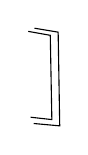
\begin{tikzpicture}[x=1cm,y=1cm]
\draw (0,1.15)--(.28,1.10)--(.30,.03)--(.03,.06);
\draw (.08,1.19)--(.38,1.14)--(.40,-.05)--(.07,-.02);
\end{tikzpicture}}}

\par\noindent 420

\scanpage{422}

\margin{les hom $\Theta,\widetilde\Theta$
$\Theta^\circ,\widetilde\Theta^\circ$}

\textcircled{\(4^\circ\)}\quad On définit un hom.
\diagram{\begin{tikzcd}[ampersand replacement=\&,column sep=huge]
\text{(57)}\quad\mathcal M_{\rho,\sigma} \arrow[r,"{\Theta}"] \& G
\end{tikzcd}}
\[
\Theta\mid\widetilde{\mathcal G}_{\rho,\sigma}^{+}\simeq SG
\quad\text{est l'identité}
\]
\[
\Theta\mid\mathcal M_{\rho,\sigma}(0)\subset
T_0\times T_\rho\times N'_\sigma
\quad\text{donné par}\quad
\Theta(\underline u,\underline a,\underline b)=\underline u
\]
d'où
\[
(58)\qquad
\Theta\mid\mathcal M_{\rho,\sigma}[0]\subset
B'_0\times T_\rho\times N'_\sigma
\quad\text{donné par}\quad
\Theta(\underline u,\underline a,\underline b)=\underline u
\]

On a
\diagram{\begin{tikzcd}[ampersand replacement=\&,column sep=large,row sep=large,nodes in empty cells]
\text{(59)}\quad\deleted{\operatorname{Ker}\Theta=}
\arrow[d,phantom,"{\deleted{\simeq}}"{description,rotate=90}]
\& \mathcal M_{\rho,\sigma}(0)
\arrow[r,phantom,"{\subset}" description]
\arrow[d,phantom,"{\cup}" description]
\arrow[dr,phantom,"{\text{cart.}}" description]
\& T_0\times T_\rho\times N'_\sigma
\arrow[d,phantom,"{\cup}" description]\\
\deleted{\unsure{\mathcal R|SG}}
\& \operatorname{Ker}\Theta
\arrow[r,phantom,"{\subset}" description]
\& 1\times T_\rho\times N'_\sigma
\end{tikzcd}}
\[
\begin{gathered}
\rotatebox{90}{$\simeq$}\quad
\left\{\left(1,
\underset{\substack{\rotatebox{90}{$\in$}\\\Gamma T_\rho}}{\underline a},
\underset{\substack{\rotatebox{90}{$\in$}\\\Gamma N'_\sigma}}{\underline b}
\right)\,\middle|\,\det\underline b=1,(\det\underline a)^2=1\right\}\\
\rotatebox{90}{$\simeq$}\quad S'T_\rho\times SN'_\sigma
\end{gathered}
\]
\inserted{où
$SN'_\sigma=\operatorname{Ker}(N'_\sigma\xrightarrow{\text{dét}}\mathbb G_m)$}

Soit
\[
(60)\qquad
\Theta^\circ=\Theta\mid\mathcal M_{\rho,\sigma}^{\circ}
\qquad\deleted{\text{\unsure{qu'on|on a}}}
\]
on trouve
\diagram{\begin{tikzcd}[ampersand replacement=\&,column sep=large,row sep=small,nodes in empty cells]
\text{(61)}\quad1 \arrow[r] \& \operatorname{Ker}\Theta^\circ
\arrow[r] \arrow[d,phantom,"{\simeq}"{description,rotate=90}]
\& \operatorname{Ker}\Theta \arrow[r,"{(\varepsilon_3,\varepsilon_2)}"]
\& \mu_2\times\mu_2 \arrow[r] \& 1.\\
\& ST_\rho\times ST_\sigma
\arrow[d,phantom,"{\deleted{\simeq}}"{description,rotate=90}] \& \& \&\\
\& \deleted{\operatorname{Centr}} \& \& \&\\[-1.5ex]
\& \deleted{\bigl(\uline{\operatorname{Rad}}(\mathcal M_{\rho,\sigma}^{\circ})}
\arrow[d,phantom,"{\deleted{\simeq}}"{description,rotate=90}] \& \& \&\\
\& \deleted{\uline{\operatorname{Centr}}^\circ(\mathcal M_{\rho,\sigma}^{\circ})\bigr)}
\& \& \&
\end{tikzcd}}

Posons
\[
(62)\qquad
S\mathcal R_{\rho,\sigma}^{\circ}
=1\times ST_\rho\times ST_\sigma
=\operatorname{Ker}\Theta^\circ
=(\operatorname{Ker}\Theta)\cap\mathcal M_{\rho,\sigma}^{\circ}
\]
qui est un sous-groupe central de $\mathcal M_{\rho,\sigma}^{\circ}$
(il est

\par\noindent 421

\scanpage{423}
\mspage{513}

\deleted{\unsure{invariant}}\inserted{distingué}
mais pas central dans $\mathcal M_{\rho,\sigma}$ tout entier)

le groupe
\[
(63)\qquad
\mathcal M_{\rho,\sigma}/S\mathcal R_{\rho,\sigma}^{\circ}
=\mathcal M_{\rho,\sigma}^{\unsure{\natural}}
\]
est donc une extension de $\mu_2\times\mu_2$ par
\[
\mathcal M_{\rho,\sigma}^{\circ}/S\mathcal R_{\rho,\sigma}^{\circ}
\overset{\mathrm{dfn}}{=}
\mathcal M_{\rho,\sigma}^{\circ\unsure{\natural}},
\]
isomorphe à $G$ par $\Theta^\circ$
(puisque $S\mathcal R_{\rho,\sigma}^{\circ}=\operatorname{Ker}\Theta^\circ$), donc
\diagram{\begin{tikzcd}[ampersand replacement=\&,column sep=large]
\text{(64)}\quad1 \arrow[r] \& G \arrow[r] \&
\mathcal M_{\rho,\sigma}^{\unsure{\natural}} \arrow[r] \&
\mu_2\times\mu_2 \arrow[r] \& 1,
\end{tikzcd}}
d'ailleurs l'hom
\diagram{\begin{tikzcd}[ampersand replacement=\&,column sep=large]
\Theta:\mathcal M_{\rho,\sigma} \arrow[r] \& G
\end{tikzcd}}
étant trivial sur $\mathcal R_{\rho,\sigma}$ passe au quotient en
\diagram{\begin{tikzcd}[ampersand replacement=\&,column sep=large]
\text{(65)}\quad\Theta^{\unsure{\natural}}:
\mathcal M_{\rho,\sigma}^{\unsure{\natural}} \arrow[r] \& G,
\end{tikzcd}}
\unsure{dont} la restriction à $G$ (via (64)) est l'identité,
donc on trouve, via (64),
\[
(66)\qquad
\mathcal M_{\rho,\sigma}^{\unsure{\natural}}\simeq
G\times\mu_2\times\mu_2.
\]
On trouve donc
\diagram{\begin{tikzcd}[ampersand replacement=\&,column sep=large,row sep=small]
\text{(67)}\quad1 \arrow[r] \& S\mathcal R_{\rho,\sigma}^{\circ}
\arrow[r] \arrow[d,phantom,"{\simeq}"{description,rotate=90}]
\& \mathcal M_{\rho,\sigma}
\arrow[r,"{(\Theta,\varepsilon_3,\varepsilon_2)}"] \&
\mathcal M_{\rho,\sigma}^{\unsure{\natural}}
\arrow[r] \arrow[d,phantom,"{\simeq}"{description,rotate=90}] \& 1.\\
\& ST_\rho\times ST_\sigma \& \& G\times\mu_2\times\mu_2 \&
\end{tikzcd}}

Pour voir comment
$\mathcal M_{\rho,\sigma}^{\unsure{\natural}}\simeq G\times\mu_2\times\mu_2$
opère sur $ST_\rho\times ST_\sigma$, on
\deleted{considère le}\inserted{note que}\deleted{l'image}
$\mathcal M_{\rho,\sigma}^{\circ}$ est l'image inverse de
$G\simeq\mathcal M_{\rho,\sigma}^{\unsure{\natural}\circ}$
\deleted{sous-groupe}
dans l'extension (67), où $S\mathcal R_{\rho,\sigma}$ est central
dans $\mathcal M_{\rho,\sigma}$, donc $G$ y opère trivialement.

\par\noindent 422


\scanpage{424}

D'autre part on a
\diagram{\begin{tikzcd}[ampersand replacement=\&,column sep=large,row sep=small]
S\mathcal R_{\rho,\sigma}^{\circ}
\arrow[r,phantom,"{\subset}"{description}]
\arrow[d,phantom,"{\simeq}"{description,rotate=90}]
\& \mathcal M_{\rho,\sigma}(0)
\arrow[r,"{\text{épi}}","{(\varepsilon_3,\varepsilon_2)}"']
\arrow[d,phantom,"{\cap}"{description}]
\& \mu_2\times\mu_2\\
ST_\rho\times ST_\sigma \& T_0\times T_\rho\times N'_\sigma \&
\end{tikzcd}}
et on trouve que $\mu_2\times\mu_2$ opère sur
$S\mathcal R_{\rho,\sigma}$ via son deuxième facteur
(correspondant à
$\varepsilon_2(\underline u,\underline a,\underline b)
=\varepsilon_\sigma(\underline b)$), un $\varepsilon$ de celui-ci
($\varepsilon^2=1$) opère sur
$S\mathcal R_{\rho,\sigma}\simeq ST_\rho\times ST_\sigma$
en laissant intouché le premier facteur,
et en opérant sur $T_\sigma$ donc sur $ST_\sigma$ via
\diagram{\begin{tikzcd}[ampersand replacement=\&,column sep=large]
\text{(68)}\qquad\sigma \arrow[r] \& \varepsilon\sigma
\end{tikzcd}}
\margin{(compatible avec l'équation de Hamilton--Cayley
$\sigma^2-\nu=0$ de $\sigma$)}

\deleted{On trouve en passant que l'image inverse
 dans $\mathcal M_{\rho,\sigma}$
\inserted{(ou $\mathcal M_{\rho,\sigma}^{\circ}$)}
du sous-groupe $\mathbb G_m\subset G$
centre de $G$ \unsure{n'est autre que}
$\mathcal M_{\rho,\sigma}^{\unsure{\circ}}(0)^\circ$.}

\textcircled{\(5^\circ\)}\quad Soit
\[
(69)\qquad
\begin{gathered}
\mathcal R_{\rho,\sigma}^{\circ}\quad
\text{image inverse de }\mathbb G_m\subset G\\
\text{dans }\mathcal M_{\rho,\sigma}^{\circ}\text{ par }
\Theta:\mathcal M_{\rho,\sigma}^{\circ}\longrightarrow G
\end{gathered}
\]

\margin{Il y aurait intérêt à \unsure{commencer}
tt de suite avec l'introduction
de $\mathcal R_{\rho,\sigma}$ et la réalisation
(102) plus bas de $\mathcal M_{\rho,\sigma}$,
en termes de sommes
amalg. des prod...\ cf
\textcircled{\(6^\circ\)}.}

On a donc une structure d'extension sur $\mathcal R_{\rho,\sigma}^{\circ}$
\diagram{\begin{tikzcd}[ampersand replacement=\&,column sep=large]
\text{(70)}\quad1 \arrow[r] \& S\mathcal R_{\rho,\sigma}^{\circ}
\arrow[r] \& \mathcal R_{\rho,\sigma}^{\circ}
\arrow[r] \& \mathbb G_m \arrow[r] \& 1.
\end{tikzcd}}
On aura
\[
\mathcal R_{\rho,\sigma}^{\circ}=
\left\{\left(
\underset{\substack{\rotatebox{90}{$\in$}\\\Gamma T_0}}{\underline u},
\underset{\substack{\rotatebox{90}{$\in$}\\\Gamma T_\rho}}{\underline a},
\underset{\substack{\rotatebox{90}{$\in$}\\\Gamma T_\sigma}}{\underline b}
\right)\cdot
\underset{\substack{\rotatebox{90}{$\in$}\\\Gamma SG}}{f}
\ \middle|\ 
\det u=\det\underline a=\det\underline b,\quad
\underline u f\in\Gamma\mathbb G_m
\right\}
\]
\inserted{i.e. $f=\lambda\underline u^{-1}$
 où $\lambda\in\Gamma\mathbb G_m$, $\lambda^2=\det u$}

\par\noindent 423

\scanpage{425}
\mspage{514}

\[
\tag{71}
\mathcal R_{\rho,\sigma}^{\circ}\simeq
\left\{\left(
 j_{T_0}(\mu^2),
 \underset{\substack{\rotatebox{90}{$\in$}\\ \Gamma T_\rho}}{\underline a},
 \underset{\substack{\rotatebox{90}{$\in$}\\ \Gamma T_\sigma}}{\underline b}
 \right)\cdot
 \underbrace{\mu j_G(\mu^{-2})}_{\inserted{\begin{gathered}
 \text{NB. le}\\[-2pt]
 \text{det est }1\\[-2pt]
 \text{car }\det j_G(\mu^{-2})=\mu^{-2}
 \end{gathered}}}
 \;\middle|\;
 \begin{gathered}
 \unsure{\mu}\in\Gamma \mathbb G_m,\\[-2pt]
 \det\underline a=\det\underline b\deleted{\unsure{=\lambda^2}}\\[-2pt]
 \underline a\in\Gamma T_\rho,\qquad=\mu^2\\[-2pt]
 \underline b\in\Gamma T_\sigma,
 \end{gathered}\right\}
\]

où \inserted{$\unsure{j^{+}|j_G}$}
\[
\tag{72}
\left\{\begin{aligned}
 j(\unsure{\mu})&=\begin{pmatrix}\mu&1\\0&1\end{pmatrix}
 \in\Gamma SG\qquad(\mu\in\Gamma \mathbb G_m)\\
 j_{T_0}\deleted{(\unsure{\mu})}&:\mathbb G_m\longrightarrow T_0
 \quad\text{donné par }j\\
 j_G&:\mathbb G_m\longrightarrow\unsure{\deleted{S}}G
 \quad\text{donné par }j\text{ précédent.}
\end{aligned}\right.
\]

On trouve ainsi que le composé
\[
\tag{73}
\left\{\begin{gathered}
\diagram{\begin{tikzcd}[ampersand replacement=\&,column sep=large]
\mathcal R_{\rho,\sigma}^{\circ}
 \arrow[r,hook,"{\text{incl}}"'] \&
\mathcal M_{\rho,\sigma}^{\circ}
 \arrow[r,"{\text{can.}}"'] \&
\begin{gathered}
\mathcal T_{\rho,\sigma}^{\circ}\simeq T_\rho\mathbin{\times}_{\mathbb G_m}T_\sigma\\
\shortparallel\\[-3pt]
\mathcal M_{\rho,\sigma}^{\circ}/\widetilde{\mathcal G}_{\rho,\sigma}^{+}
\end{gathered}
\end{tikzcd}}\\
\text{fait de }\mathcal R_{\rho,\sigma}^{\circ}
 \text{ un revêtement \unsure{algébrique}}\\
\text{de }\mathcal T_{\rho,\sigma}^{\circ}
\end{gathered}\right.
\]

et plus précisément qu'on a un diagramme cartésien
\[
\tag{74}
\diagram{\begin{tikzcd}[ampersand replacement=\&,column sep=huge,row sep=large]
\mathcal R_{\rho,\sigma}^{\circ}
 \arrow[r,"{(73)}"]
 \arrow[d,"{\substack{\text{l'hom. can.}\\\text{de }(70)}}"']
 \arrow[dr,phantom,"{\text{cart}}",description] \&
T_\rho\mathbin{\times}_{\mathbb G_m}T_\sigma\simeq\mathcal T_{\rho,\sigma}^{\circ}
 \arrow[d,"{\text{can}}"]\\
\mathbb G_m \arrow[r,"{\mu\longmapsto\mu^2}"'] \&\mathbb G_m
\end{tikzcd}}
\]

\noindent(75)\quad\uline{Proposition} :
$\mathcal R_{\rho,\sigma}^{\circ}=\uline{Centr}(\mathcal M_{\rho,\sigma}^{\circ})$

Évidemment le centre de $\mathcal M_{\rho,\sigma}^{\circ}$ est contenu
 dans $\mathcal R_{\rho,\sigma}^{\circ}$, image inverse justement du centre

\par\noindent 424

\scanpage{426}

de $\mathcal M_{\rho,\sigma}^{\circ\unsure{\natural|\sharp}}
 =\mathcal M_{\rho,\sigma}^{\circ}/S\mathcal R_{\rho,\sigma}\simeq G$,
 il reste à prouver que $\mathcal R_{\rho,\sigma}$ est central dans
 $\mathcal M_{\rho,\sigma}^{\circ}$.
Mais \deleted{pour un élément} $\mathcal M_{\rho,\sigma}^{\circ}$ est
 engendré \deleted{$(\underline u,\underline a,\underline b\unsure{)}$}
 par $\mathcal R_{\rho,\sigma}^{\circ}$ et par
 $\widetilde{\mathcal G}_{\rho,\sigma}^{+}\simeq SG$,
 puisque
\[
\diagram{\begin{tikzcd}[ampersand replacement=\&,column sep=large]
\mathcal R_{\rho,\sigma}^{\circ}\arrow[r]\&
\mathcal T_{\rho,\sigma}^{\circ}\simeq
\mathcal M_{\rho,\sigma}^{\circ}/\widetilde{\mathcal G}_{\rho,\sigma}^{+}
\end{tikzcd}}
\]
 est épi (73)(74), et comme $\mathcal R_{\rho,\sigma}$ est commutatif
 (74), il reste à montrer qu'il commute à
 $\widetilde{\mathcal G}_{\rho,\sigma}^{+}$ i.e. opère trivialement sur
 $\widetilde{\mathcal G}_{\rho,\sigma}^{+}$.
Or une section de $\mathcal R_{\rho,\sigma}^{\circ}$ est de la forme
\[
 (j_{T_0}(\mu^2),\underline a,\underline b)\cdot
 (\lambda j_{\unsure{T_0}}(\mu^{-2}))
\]
le premier facteur opérant comme \deleted{$\operatorname{int}$}
\[
 \unsure{i.}\qquad\operatorname{int}j_G(\mu^2)
\]
le deuxième comme
\[
 \operatorname{int}j_G(\mu^{\unsure{-2}})
\]
donc leur produit opère trivialement, cqfd

\deleted{Notons \unsure{en}} \inserted{Notons maintenant que}
\[
\tag{75}
\mathcal R_{\rho,\sigma}^{\circ}\cap
 \underbrace{\widetilde{\mathcal G}_{\rho,\sigma}^{+}}_{\substack{\shortparallel\\ SG}}
 =\operatorname{Ker}(\mathcal R_{\rho,\sigma}^{\circ}\longrightarrow
 \mathcal T_{\rho,\sigma}^{\circ})
 \underset{\substack{\big|\\\text{cf }(74)}}{=}\mu_2
\]
(on peut dire aussi plus directement, que

\par\noindent 425

\scanpage{427}
\mspage{515}

$\mathcal R_{\rho,\sigma}^{\circ}\cap\widetilde{\mathcal G}_{\rho,\sigma}^{+}$,
 étant contenu dans le centre de
 $\widetilde{\mathcal G}_{\rho,\sigma}^{+}\simeq SG$ qui est $\mu_2$,
 est $\subset\mu_2$ --- mais cela ne montre pas l'égalité.

\uline{Rmq} Cela donne une description plus simple de
 $\mathcal M_{\rho,\sigma}^{\circ}$ que comme produit $\frac12$ direct,
 de la façon suivante. On définit $\mathcal R_{\rho,\sigma}^{\circ}$
 par le diagramme (74), d'où une suite exacte
\[
\tag{77}
\diagram{\begin{tikzcd}[ampersand replacement=\&,column sep=large]
1\arrow[r]\&\mu_2\arrow[r,"{j'}"]\&
\mathcal R_{\rho,\sigma}^{\circ}\arrow[r]\&
T_\rho\mathbin{\times}_{\mathbb G_m}T_\sigma\arrow[r]\&1
\end{tikzcd}}
\]
et on définit $\mathcal M_{\rho,\sigma}^{\circ}$ comme somme
 \unsure{amalgamée} centrale
\[
\deleted{(78)\qquad\unsure{\mathcal M_{\rho,\sigma}^{\circ}}}
\]
\[
\tag{78}
\diagram{\begin{tikzcd}[ampersand replacement=\&,column sep=large,row sep=small]
1\arrow[r]\&\mu_2\arrow[r]\&
\mathcal R_{\rho,\sigma}^{\circ}\times
 \begin{gathered}
 \deleted{\unsure{\mathcal M}}\inserted{\widetilde{\mathcal G}}_{\rho,\sigma}^{+}\\
 \shortparallel\\[-3pt] SG
 \end{gathered}
 \arrow[r]\&\mathcal M_{\rho,\sigma}^{\circ}\arrow[r]\&1\\
\&\varepsilon\arrow[r,mapsto]\&(j'(\varepsilon),j''(\varepsilon^{-1}))\&\&
\end{tikzcd}}
\]
(où $j'$ est donné dans (77) et
 $j'':\mu_2\longrightarrow SG=\widetilde{\mathcal G}_{\rho,\sigma}^{+}$
 le morph. can.).

Notons qu'on a de $=$ une
 \deleted{\unsure{bien con.}}\inserted{description} bien connue de $G$
 en termes de $SG$
\[
\tag{79}
\diagram{\begin{tikzcd}[ampersand replacement=\&,column sep=large,row sep=small]
1\arrow[r]\&\mu_2\arrow[r]\&\mathbb G_m\times SG\arrow[r]\&G\arrow[r]\&1\\
\&\varepsilon\arrow[r,mapsto]\&(\varepsilon,j''(\varepsilon^{-1}))\&\&
\end{tikzcd}}
\]
et on aura un hom de (78) dans (79),
 grâce à l'hom can
\[
\tag{80}
\diagram{\begin{tikzcd}[ampersand replacement=\&,column sep=large]
\mathcal R_{\rho,\sigma}^{\circ}\arrow[r]\&\mathbb G_m
\end{tikzcd}}
\qquad\text{de }(74),
\]

\par\noindent 426

\scanpage{428}

ce qui par passage au quotient \unsure{dans|des}
\[
\diagram{\begin{tikzcd}[ampersand replacement=\&,column sep=large]
\mathcal R_{\rho,\sigma}^{\circ}\times SG
 \arrow[r,"{\widetilde\Theta^{\circ}}"] \&\mathbb G_m\times SG
\end{tikzcd}}
\]
permet de reconstituer
\[
\Theta^{\circ}:\quad
\diagram{\begin{tikzcd}[ampersand replacement=\&,column sep=large]
\mathcal M_{\rho,\sigma}^{\circ}\arrow[r]\&G
\end{tikzcd}},
\]
tout comme le groupe $\mathcal M_{\rho,\sigma}^{\circ}$
 lui-$=$, en termes des \inserted{schémas en}
 groupes ($\pm$ toriques) ``en l'air'' $T_\rho,T_\sigma$ et des épimorphismes
\[
\diagram{\begin{tikzcd}[ampersand replacement=\&,column sep=large]
T_\rho\arrow[r,"{\delta_\rho}"]\&\mathbb G_m
\end{tikzcd}},\qquad
\diagram{\begin{tikzcd}[ampersand replacement=\&,column sep=large]
T_\sigma\arrow[r,"{\delta_\sigma}"]\&\mathbb G_m
\end{tikzcd}},
\]
et de la forme $G$ de $\mathrm{Gl}(2)_S$ bien sûr
 (sans avoir à utiliser $=$ des plongements
 $T_\rho\longrightarrow G,T_\sigma\longrightarrow G$,
 et encore moins des sections $\rho,\sigma$ de $G\ldots$).
On \inserted{trouve $\widetilde{\mathcal G}_{\rho,\sigma}^{+}$
 comme image de $SG$, dans $\mathcal M_{\rho,\sigma}^{\circ}$,}
\deleted{et $\mathcal T_{\rho,\sigma}^{\circ}\simeq$}
\deleted{\illegible{1} \unsure{cependant} que pour notre propos,
 le \unsure{prisme|produit} des sous-groupes}
\[
\mathcal T_{\rho,\sigma}^{\circ}\overset{\mathrm{dfn}}{=}
 \mathcal M_{\rho,\sigma}^{\circ}/\widetilde{\mathcal G}_{\rho,\sigma}^{+}
 \simeq\begin{gathered}
 \mathcal R_{\rho,\sigma}^{\circ}/\mu_2\\[-2pt]
 \rotatebox{90}{$\simeq$}\\[-2pt]
 T_\rho\mathbin{\times}_{\mathbb G_m}T_\sigma
 \end{gathered}
\]

Mais pour notre propos, le scindage
 \inserted{``de travers''}
 de l'extension ainsi construite de $\mathcal T_{\rho,\sigma}^{\circ}$
 par $\widetilde{\mathcal G}_{\rho,\sigma}^{+}\simeq SG$,
 correspondant au ss-groupe section $\mathcal M_{\rho,\sigma}^{\circ}(0)$,
 jouera un rôle essentiel --- en composant cette section

\par\noindent 427

\scanpage{429}
\mspage{516}

\[
\diagram{\begin{tikzcd}[ampersand replacement=\&,column sep=large]
\mathcal T_{\rho,\sigma}^{\circ}\simeq
 T_\rho\mathbin{\times}_{\mathbb G_m}T_\sigma\arrow[r]\&
\mathcal M_{\rho,\sigma}^{\circ}
\end{tikzcd}}
\]
avec
\[
\diagram{\begin{tikzcd}[ampersand replacement=\&,column sep=large]
\mathcal M_{\rho,\sigma}^{\circ}\arrow[r]\&G
\end{tikzcd}}
\]
on trouve un homomorphisme qui se \unsure{factorise} à son tour en
\[
\diagram{\begin{tikzcd}[ampersand replacement=\&,column sep=large]
\mathcal T_{\rho,\sigma}^{\circ}\simeq
 T_\rho\mathbin{\times}_{\mathbb G_m}T_\sigma
 \arrow[r,"{\substack{\text{épi}\\\text{can}}}"]\&
\mathbb G_m\arrow[r,hook,"{\substack{\text{mono}\\j_G}}"]\&G
\end{tikzcd}}
\]
dont l'image est le tore $T_0\ldots$ .

\uline{Remarque} On peut songer à construire
 $\mathcal M_{\rho,\sigma}$ de façon \unsure{analogue}, en introduisant
 l'image inverse --- notons le
 $\mathcal R_{\rho,\sigma}^{\inserted{\unsure{\sim|\infty}}}$ --- de
 $\unsure{\mathbb G_m}\times\mu_2\times\mu_2$ par
\[
\diagram{\begin{tikzcd}[ampersand replacement=\&,column sep=large]
\mathcal M_{\rho,\sigma}\arrow[r]\&G\times\mu_2\times\mu_2
\end{tikzcd}}
\]
(67) --- dont l'intersection avec
 $\widetilde{\mathcal G}_{\rho,\sigma}^{+}\simeq SG$
 évidemment égale à $\mu_2$, puisque

\margin{\uline{NB} $\mathcal R_{\rho,\sigma}$ est aussi,
 plus simplement, le noyau de l'hom composé
\[
\widetilde\Theta:\quad
\diagram{\begin{tikzcd}[ampersand replacement=\&,column sep=large]
\mathcal M_{\rho,\sigma}\arrow[r,"{\Theta}"]\&G\arrow[r,"{\text{can}}"]\&PG
\end{tikzcd}}
\]
donc on a suite exacte
\[
\deleted{\illegible{1}}\quad(81)\qquad
\diagram{\begin{tikzcd}[ampersand replacement=\&,column sep=large]
1\arrow[r]\&\mathcal R_{\rho,\sigma}\arrow[r]\&
\mathcal M_{\rho,\sigma}\arrow[r]\&PG\arrow[r]\&1
\end{tikzcd}}
\]}

\[
\mathcal R_{\rho,\sigma}^{\circ}
 =\mathcal R_{\rho,\sigma}^{\inserted{\unsure{\sim|\infty}}}
  \cap\mathcal M_{\rho,\sigma}^{\circ}
 =(\mathcal R_{\rho,\sigma}^{\inserted{\unsure{\sim|\infty}}})^{\circ}
 \quad\inserted{\text{(composante neutre)}}
\]
\deleted{(en fait il faudrait peut-être noter
 $\mathcal R_{\rho,\sigma}^{\sim}$ plutôt $\mathcal R_{\rho,\sigma}$,
 et l'ancien $\mathcal R_{\rho,\sigma}$ deviendrait
 $\mathcal R_{\rho,\sigma}^{\circ}$, de $=$
 $S\mathcal R_{\rho,\sigma}$ deviendrait $S\mathcal R_{\rho,\sigma}^{\circ}\ldots$).}

Je ne vais pas expliciter ici la construction de
 $\mathcal R_{\rho,\sigma}^{\inserted{\unsure{\sim|\infty}}}$ en termes de
 $T_\rho,N'_\sigma$ etc, n'étant pas sûr qu'il y en aura besoin par la suite.

\par\noindent 428

\scanpage{430}

Dans le cas modulaire, sur la base absolue $\mathbb Z$, on aura

\[
(81)\quad\left(
\diagram{\begin{tikzcd}[ampersand replacement=\&,column sep=small]
\begin{array}[t]{c}S\mathcal R_{\rho,\sigma}^{\circ}(\mathbb Z)\\ \Vert\\ ST_\rho(\mathbb Z)\times ST_\sigma(\mathbb Z)\end{array}
\arrow[r,"{\sim}"] \&
\mathcal T_{\rho,\sigma}^{\circ}(\mathbb Z)\arrow[r,"{\sim}"] \&
\begin{array}[t]{c}T_\rho(\mathbb Z)\times T_\sigma(\mathbb Z)\simeq\mathbb Z/6\mathbb Z\times\mathbb Z/4\mathbb Z\\
\text{car }T_\rho(\mathbb Z)=ST_\rho(\mathbb Z)\\
T_\sigma(\mathbb Z)=ST_\sigma(\mathbb Z)\end{array}
\end{tikzcd}}\right.
\]

d'où, via (74)
\[
(82)\qquad\mathcal R_{\rho,\sigma}^{\circ}(\mathbb Z)\simeq
(\mathbb Z/6\mathbb Z\times\mathbb Z/4\mathbb Z)\times\{\pm1\}
\]

les \deleted{deux} projections sur les deux facteurs du second mb. correspondent justement aux hom
\[
\diagram{\begin{tikzcd}[ampersand replacement=\&]
\mathcal R_{\rho,\sigma}^{\circ}\arrow[r]\&\mathcal T_{\rho,\sigma}^{\circ}
\end{tikzcd}},\qquad
\diagram{\begin{tikzcd}[ampersand replacement=\&]
\mathcal R_{\rho,\sigma}^{\circ}\arrow[r]\&\mathbb G_m
\end{tikzcd}}
\]
de (74), de sorte que l'inclusion
\[
(83)\quad
\diagram{\begin{tikzcd}[ampersand replacement=\&,column sep=small]
\mu_2(\mathbb Z)=\{\pm1\}\arrow[r]\&
\mathcal R_{\rho,\sigma}^{\circ}(\mathbb Z)\simeq
(\mathbb Z/6\mathbb Z\times\mathbb Z/4\mathbb Z)\times\{\pm1\}
\end{tikzcd}}
\]
est l'inclusion évidente
$\varepsilon\longmapsto(0)\times\varepsilon$.

Une façon plus \unsure{parlante} de dire ceci est que l'inclusion canonique
\[
(84)\quad
\diagram{\begin{tikzcd}[ampersand replacement=\&,column sep=small]
\begin{array}[t]{c}S\mathcal R_{\rho,\sigma}^{\circ}\\\Vert\\
ST_\rho\times ST_\sigma\\\cap\\
\unsure{1}\,\mathcal M_{\rho,\sigma}^{\circ}(0)\end{array}
\times
\begin{array}[t]{c}\mu_2\\\deleted{\unsure{\mathbb G_m}}\\\Vert\\
\text{\uline{Centr}}(SG)\end{array}
\arrow[r,hook]\&\mathcal R_{\rho,\sigma}^{\circ}
\end{tikzcd}}
\]
induit un \uline{isomorphisme}
\[
(85)\quad
\diagram{\begin{tikzcd}[ampersand replacement=\&,column sep=large]
\underbrace{S\mathcal R_{\rho,\sigma}^{\circ}(\mathbb Z)}_{\mathbb Z/6\mathbb Z\times\mathbb Z/4\mathbb Z}
\times
\underbrace{\mu_2(\mathbb Z)}_{\{\pm1\}}
\arrow[r,"{\sim}"]\&\mathcal R_{\rho,\sigma}^{\circ}(\mathbb Z)
\end{tikzcd}}
\]

\par\noindent 429

\scanpage{431}
\mspage{517}

\deleted{\textcircled{$6^{\circ}$}\quad\uline{Le \unsure{sous-groupe}} $\mathcal M_{\rho,\sigma}(\unsure{\tfrac12})$}

\margin{\uline{\unsure{Groupes mixtes}}\par
\uline{du radical}\par
$(\mathcal R_{\rho,\sigma},S\mathcal R_{\rho,\sigma},\mathcal R_{\rho,\sigma}^{\circ},
S\mathcal R_{\rho,\sigma}^{\circ}\ldots)$.}

\textcircled{$6^{\circ}$}\quad Je vais revenir sur
\[
(86)\qquad
\mathcal R_{\rho,\sigma}\overset{\mathrm{dfn}}=
\operatorname{Ker}\left(
\diagram{\begin{tikzcd}[ampersand replacement=\&]
\mathcal M_{\rho,\sigma}\arrow[r,"{\widetilde\Theta}"]\&PG
\end{tikzcd}}\right),
\]
donnant lieu à la suite exacte
\[
(87)\quad\diagram{\begin{tikzcd}[ampersand replacement=\&]
1\arrow[r,no head]\&\mathcal R_{\rho,\sigma}\arrow[r]\&
\mathcal M_{\rho,\sigma}\arrow[r,no head]\&PG\arrow[r,no head]\&1.
\end{tikzcd}}
\]
On aura
\[
(88)\qquad
\underset{\inserted{\substack{\text{défini}\\\text{dans 69}}}}{\mathcal R_{\rho,\sigma}^{\circ}}
=\mathcal R_{\rho,\sigma}\cap\mathcal M_{\rho,\sigma}^{\circ}
=\begin{array}[t]{c}\text{comp. neutre}\\\text{de }\mathcal R_{\rho,\sigma}\end{array}.
\]

\unsure{Dailleurs} on a aussi
\[
(89)\qquad\mathcal R_{\rho,\sigma}=\Theta^{-1}(\mathbb G_m)
\qquad\left(\Theta:\diagram{\begin{tikzcd}[ampersand replacement=\&]
\mathcal M_{\rho,\sigma}\arrow[r]\&G
\end{tikzcd}}\right)
\]
d'où une suite exacte
\[
(90)\quad\diagram{\begin{tikzcd}[ampersand replacement=\&,column sep=small]
1\arrow[r]\&
\begin{array}[t]{c}S\mathcal R_{\rho,\sigma}\\
\inserted{\Vert\,\mathrm{dfn}}\\
\inserted{\left\{\begin{array}{l}
\operatorname{Ker}\,\deleted{\unsure{\kappa|\Theta}}
(\mathcal R_{\rho,\sigma}\xrightarrow{\kappa}\mathbb G_m)\\
\Vert\\
\operatorname{Ker}(\mathcal M_{\rho,\sigma}\xrightarrow{\Theta}G)
\end{array}\right.}
\end{array}
\arrow[r]\&\mathcal R_{\rho,\sigma}\arrow[r,"{\kappa}"]\&\mathbb G_m\arrow[r]\&1
\end{tikzcd}}
\]
où $\kappa$ est défini par la condition que
\[
(91)\quad\diagram{\begin{tikzcd}[ampersand replacement=\&,column sep=small]
\mathcal R_{\rho,\sigma}\arrow[r,"{\kappa}"]
\arrow[rrr,bend right=25,"{\Theta}"']\&
\mathbb G_m\arrow[r,"{\sim}"]\&\text{\uline{Centr}}(G)\arrow[r]\&G
\end{tikzcd}}
\]
soit commutatif.

Notons en passant que l'hom $\chi$ de (42)
$\mathcal M_{\rho,\sigma}\longrightarrow \mathbb G_m$ peut se déduire aussi de $\Theta$
(57) p- composition
\[
(92)\quad\diagram{\begin{tikzcd}[ampersand replacement=\&,column sep=small]
\mathcal M_{\rho,\sigma}\arrow[rr,"{\Theta}"]\arrow[dr,"{\chi}"']\&\&G\arrow[dl,"{\det}"]\\
\&\mathbb G_m\&
\end{tikzcd}}\quad\unsure{)|,}
\]
et on aura donc
\[
(93)\qquad\chi(g)=\kappa(g)^2\quad\text{si }g\in\Gamma\mathcal R_{\rho,\sigma}
\]
i.e.
\[
\diagram{\begin{tikzcd}[ampersand replacement=\&,column sep=small]
\mathcal R_{\rho,\sigma}\arrow[rr,"{\kappa}"]
\arrow[dr,"{\chi|\mathcal R_{\rho,\sigma}}"']\&\&\mathbb G_m\arrow[dl,"{\lambda\mapsto\lambda^2}"]\\
\&\mathbb G_m\,\deleted{\unsure{\mathbb G_m}}\&
\end{tikzcd}}
\qquad\text{commutatif.}
\]

\par\noindent 430

\scanpage{432}

On a le diagramme d'inclusions
\[
(94)\quad
\diagram{\begin{tikzcd}[ampersand replacement=\&,
row sep=6em,column sep=8em,
execute at end picture={
\node[anchor=south] at (sra.north) {$(90)$};
\node[anchor=south] at (ra.north) {$(86)$};
\node[anchor=north west] at (sra.south east) {$=\operatorname{Ker}\Theta$};
\node[anchor=north west] at (ra.south east) {$=\operatorname{Ker}\widetilde\Theta$};
\node[anchor=north] at ([yshift=-1.6em]sroa.south) {$(62)$};
\node[anchor=north west] at (sroa.south east) {$=\operatorname{Ker}\Theta^{\circ}$};
\node[anchor=north east] at ([xshift=-.5em,yshift=-.5em]sroa.south west) {$ST_\rho\times ST_\sigma$};
\node[rotate=45] at ([xshift=-.3em,yshift=-.2em]sroa.south west) {$=$};
\node[anchor=north] at ([yshift=-1.6em]roa.south) {$(69)$};
\node[anchor=north west] at (roa.south east) {$=\operatorname{Ker}\widetilde\Theta^{\circ}$};
}]
|[alias=sra]|S\mathcal R_{\rho,\sigma}
\arrow[r,hook,"{\mathbb G_m}"]
\arrow[dr,phantom,"{{\begin{array}{c}\text{cart}\\\text{et cocart}\end{array}}}" description]\&
|[alias=ra]|\mathcal R_{\rho,\sigma}
\arrow[r,hook,"{PG}"]
\arrow[dr,phantom,"{{\begin{array}{c}\text{cart et}\\\text{cocart}\end{array}}}" description]\&
\mathcal M_{\rho,\sigma}\\
|[alias=sroa]|S\mathcal R_{\rho,\sigma}^{\circ}
\arrow[u,hook,"{\mu_2\times\mu_2}"]\arrow[r,hook,"{\mathbb G_m}"]\&
|[alias=roa]|\mathcal R_{\rho,\sigma}^{\circ}
\arrow[u,hook,"{\mu_2\times\mu_2}"]
\arrow[r,hook,"{PG}","{\unsure{1}}"']\&
\mathcal M_{\rho,\sigma}^{\circ}\arrow[u,hook,"{\mu_2\times\mu_2}"']
\end{tikzcd}}
\]

\margin{NB\par
Il y a une vérification à faire, qui se réduit à voir que
\[
\diagram{\begin{tikzcd}[ampersand replacement=\&,column sep=small]
S\mathcal R_{\rho,\sigma}\arrow[r]\&\mu_2\times\mu_2
\end{tikzcd}}
\quad\text{est épi}
\]
(son noyau est $S\mathcal R_{\rho,\sigma}^{\circ}$ par déf),
donc à fortiori
\[
\diagram{\begin{tikzcd}[ampersand replacement=\&,column sep=small]
\mathcal R_{\rho,\sigma}\arrow[r,no head]\&\mu_2\times\mu_2
\end{tikzcd}}\quad\text{épi}
\]
(son noyau est $\mathcal R_{\rho,\sigma}^{\circ}$ par définition)
--- mais la vérification est triviale.}

la deuxième ligne est formée des composantes neutres de la première, qu'on peut réécrire plus joliment encore
\[
(95)\quad
\diagram{\begin{tikzcd}[ampersand replacement=\&,row sep=1.4em,column sep=1.4em]
\&\&\mathcal R_{\rho,\sigma}\arrow[drrr,hook,"{PG}"]\&\&\&\\
S\mathcal R_{\rho,\sigma}\arrow[urr,hook,"{\mathbb G_m}"]
\arrow[rrrrr,"{{\deleted{\unsure{G}}\quad G}}"]
\arrow[drrr,dashed,no head]\&\&\&\&\&\mathcal M_{\rho,\sigma}\\
\&\&\&\inserted{\mathcal M_{\rho,\sigma}^{+}}
\arrow[urr,dashed,no head]\&\&\\
\&\&S\mathcal R_{\rho,\sigma}
\arrow[uuu,hook,"{\mu_2\times\mu_2}"']
\arrow[drrr,hook,"{PG}"]\&\&\&\\
\begin{array}{c}S\mathcal R_{\rho,\sigma}^{\circ}\\\Vert\\(ST_\rho\times ST_\sigma)\end{array}
\arrow[uuu,hook,"{\mu_2\times\mu_2}"]
\arrow[urr,hook,"{\mathbb G_m}"]\arrow[rrrrr,"{G}"]
\arrow[drrr,dashed,no head]\&\&\&\&\&
\mathcal M_{\rho,\sigma}^{\circ}\arrow[uuu,hook,"{\mu_2\times\mu_2}"]\\
\&\&\&\inserted{\mathcal M_{\rho,\sigma}^{+\circ}}
\arrow[uuu,dashed,no head]\arrow[urr,dashed,no head]\&\&
\end{tikzcd}},
\]
sous forme d'un prisme dont les trois carrés latéraux sont à la fois cartésiens et cocartésiens --- donc donnant lieu à des quotients (sur des côtés parallèles), isomorphes --- les quotients qui interviennent sont
\[
\mu_2\times\mu_2,\quad \mathbb G_m,\quad PG\quad
\text{et l'extension }G\text{ de }PG\text{ par }\mathbb G_m.
\]
On lit sur ce diagramme, p.ex., la suite exacte
\[
(96)\quad
\diagram{\begin{tikzcd}[ampersand replacement=\&,column sep=small]
1\arrow[r]\&
\begin{array}[t]{c}S\mathcal R_{\rho,\sigma}^{\circ}\\\simeq\\ST_\rho\times ST_\sigma\end{array}
\arrow[r]\&\mathcal R_{\rho,\sigma}
\arrow[r,"{{(\kappa,\varepsilon_3|\mathcal R_{\rho,\sigma},\varepsilon_2|\mathcal R_{\rho,\sigma})}}"{yshift=.3ex}]\&[7em]
\mathbb G_m\times\mu_2\times\mu_2\arrow[r]\&1
\end{tikzcd}},
\]

\par\noindent 431

\scanpage{433}
\mspage{518}

qui explicite la structure de $\mathcal R_{\rho,\sigma}$ en termes des groupes très simples $ST_\rho,ST_\sigma,\mathbb G_m,\mu_2$.

On a un cube, construit sur la face verticale postérieure gauche de (95) (qui devient la face \deleted{post} verticale postérieure)
\[
(95)\quad
\diagram{\begin{tikzcd}[ampersand replacement=\&,row sep=4em,column sep=2.6em]
S\mathcal R_{\rho,\sigma}
\arrow[rr,hook,"{\mathbb G_m}"]
\arrow[dr,line width=1pt,"{\deleted{\unsure{\mu_2}}}","{\unsure{\simeq}}"']\&\&
\mathcal R_{\rho,\sigma}\arrow[dr,"{\mu_2}"]\arrow[rr,dashed]\&\&
\mathbb G_m\arrow[dr,dashed,"{\lambda\mapsto\lambda^2}"]\&\\
\&\deleted{\unsure{S}}\mathcal T_{\rho,\sigma}^{+}\arrow[rr,hook,"{\mathbb G_m}"{pos=.70}]\&\&
\mathcal T_{\rho,\sigma}\arrow[rr,dashed]\&\&\mathbb G_m\\
S\mathcal R_{\rho,\sigma}^{\circ}\arrow[uu,hook,"{\mu_2\times\mu_2}"{pos=.70}]
\arrow[rr,hook,"{\mathbb G_m}"{pos=.70}]
\arrow[dr,hook,"{\deleted{\unsure{\mu_2}}}","{\unsure{\sim|\simeq}}"']\&\&
\mathcal R_{\rho,\sigma}^{\circ}\arrow[uu,hook,"{\mu_2\times\mu_2}"{pos=.70}]
\arrow[dr,"{\mu_2}"]\arrow[rr,dashed]\&\&
\mathbb G_m\arrow[uu,dashed,no head,"{\Vert}"{pos=.70}]
\arrow[dr,dashed,"{\lambda\mapsto\lambda^2}"]\&\\
\&\mathcal T_{\rho,\sigma}^{+\circ}\arrow[uu,hook,"{\mu_2\times\mu_2}"{pos=.70}]
\arrow[rr,"{\mathbb G_m}"]\&\&
\mathcal T_{\rho,\sigma}^{\circ}\arrow[uu,hook,"{\mu_2\times\mu_2}"{pos=.70}]
\arrow[rr,dotted,no head]\&\&\mathbb G_m\arrow[uu,dotted,no head,"{\Vert}"{pos=.70}]
\end{tikzcd}};
\]
dont les faces \inserted{verticales} postérieure (contenue aussi dans (95)) et antérieure sont cartésiennes et cocartésiennes, et les \inserted{4} flèches horizontales qui vont de celle-là à celle-ci sont des morphismes de passage au quotient, ayant tous des noyaux isomorphes \inserted{soit à} $\mu_2$ (marqués au dessus de ces flèches), soit à $1$
(\deleted{\unsure{marqués par}}
\inserted{\deleted{\unsure{autrefois}}\unsure{on en fait}}
des flèches \deleted{\unsure{d'inclusion|d'isomorphisme} $\longrightarrow$}
\inserted{qui sont des iso $\xrightarrow{\sim}$}),
ce qui \deleted{\unsure{qui implique les relations}}
\unsure{exprime|explicite|implique} les relations,
\[
(97)\qquad
\left\{
\begin{aligned}
\deleted{S}\mathcal R_{\rho,\sigma}\cap SG
&=\deleted{\unsure{S\mathcal R_{\rho,\sigma}^{\circ}\cap SG}}
\mathcal R_{\rho,\sigma}^{\circ}\cap SG
=\deleted{\unsure{S\mathcal R_{\rho,\sigma}^{\circ}\cap SG}}
\inserted{\mu_2}\,\deleted{\unsure{\mu_2}}\\
S\mathcal R_{\rho,\sigma}\cap SG
&=S\mathcal R_{\rho,\sigma}^{\circ}\cap SG=\{1\}.
\quad\deleted{\unsure{\ne\mu_2}\,(\text{\unsure{centre}}\,SG)}
\end{aligned}\right.
\]

\deleted{Pour la \deleted{première}\inserted{première ligne},
\unsure{il suffit de voir que les|il faut voir que les}
deux termes extrêmes de la première ligne sont égaux \deleted{à $\mu_2$}
et \unsure{égaux|isom.} à $\mu_2$. Or on a \unsure{évidemment}
\[
\mu_2=
\underbrace{S\mathcal R_{\rho,\sigma}^{\circ}\cap SG}_{\unsure{\operatorname{Ker}\Theta}}
\subset\deleted{S}\mathcal R_{\rho,\sigma}\cap SG
\]
}

\par\noindent 432

\scanpage{434}
\mspage{\deleted{\unsure{8}}519}

on note
\[
\underbrace{\mathcal R_{\rho,\sigma}^{\deleted{\unsure{\circ}}}}_{\operatorname{Ker}\widetilde\Theta}
\cap SG=\operatorname{Ker}(\widetilde\Theta|SG),\qquad
\underbrace{\mathcal R_{\rho,\sigma}^{\circ}}_{\operatorname{Ker}\widetilde\Theta^{\circ}}
\cap SG=\operatorname{Ker}(\widetilde\Theta^{\circ}|SG),
\]
or
\[
\widetilde\Theta|SG=\widetilde\Theta^{\circ}|SG
=\text{morphisme can. }\diagram{\begin{tikzcd}[ampersand replacement=\&]SG\arrow[r]\&PG\end{tikzcd}}
\]
dont le noyau est bien $\mu_2$.

D'autre part on a
\[
\underbrace{S\mathcal R_{\rho,\sigma}}_{\operatorname{Ker}\Theta}
\cap SG=\operatorname{Ker}(\Theta|SG)=\{1\}
\]
puisque $\Theta|SG$ est l'inclusion can. $SG\subset G$,
a fortiori $S\mathcal R_{\rho,\sigma}^{\circ}\cap SG=\{1\}$.
Le fait que l'on a des \uline{isomorphismes}
\[
(98)\qquad\left\{\begin{array}{l}
\diagram{\begin{tikzcd}[ampersand replacement=\&,column sep=small]
S\mathcal R_{\rho,\sigma}\arrow[r,"{\sim}"]\&
\mathcal T_{\rho,\sigma}^{+}\simeq S'T_\rho\times SN'_\sigma
\end{tikzcd}}\\[1.5em]
\diagram{\begin{tikzcd}[ampersand replacement=\&,column sep=small]
S\mathcal R_{\rho,\sigma}^{\circ}\arrow[r,"{\sim}"]\&
\mathcal T_{\rho,\sigma}^{+\circ}\simeq ST_\rho\times ST_\sigma
\end{tikzcd}}
\end{array}\right.
\]
résulte, \deleted{\unsure{de}} pour le deuxième, de la comparaison
de (62) et de (28), pour le premier cela s'en
déduit par le lemme des cinq, puisque
\[
\diagram{\begin{tikzcd}[ampersand replacement=\&,column sep=large]
S\mathcal R_{\rho,\sigma}/S\mathcal R_{\rho,\sigma}^{\circ}
\arrow[r,"{\sim}"]\&
\mathcal T_{\rho,\sigma}^{+}/\mathcal T_{\rho,\sigma}^{+\circ}
\simeq\mu_2\times\mu_2.
\end{tikzcd}}
\]

Le fait que \deleted{$\unsure{S\mathcal R_\rho}$} l'on ait des \uline{iso} (98)
implique que dans
\[
\underset{\substack{\Vert\,\mathrm{dfn}\\
\unsure{\operatorname{Ker}|\operatorname{Ker}'}
(\chi:\mathcal M_{\rho,\sigma}\to \mathbb G_m)}}{\mathcal M_{\rho,\sigma}^{+}}
\simeq
\underbrace{\mathcal M_{\rho,\sigma}^{+}(0)}_{\simeq\mathcal T_{\rho,\sigma}^{+}}
\mathbin{.}
\underbrace{\widetilde{\mathcal G}_{\rho,\sigma}^{+}}_{SG}
\qquad\begin{array}{c}(\text{produit }\tfrac12\text{ direct}\\\text{cf (44)})\end{array}
\]
regardé comme extension de $\mathcal T_{\rho,\sigma}^{+}$ par $SG$,
il y a, à côté du scindage par $\mathcal M_{\rho,\sigma}^{+}(0)\subset\mathcal M_{\rho,\sigma}^{+}$,
induit par $\mathcal M_{\rho,\sigma}(0)$, un autre, scindage,

\par\noindent 433
